% this is python generate latex code , do not edit it !!

\documentclass{standalone}
\usepackage{tikz}

\usetikzlibrary{automata, positioning}
\newcommand{\createNode}[6]{\node[state,text=#5,fill=#6] at (#3,#4)(#1){#2};}
\newcommand{\createEdge}[5]{\draw[every loop,bend right,auto=right,text=#4,fill=#5](#1)edge node{#3} (#2);}
\newcommand{\createLoop}[4]{\draw[every loop,loop above,text=#3,fill=#4](#1)edge node{#2} (#1);}

\begin{document}
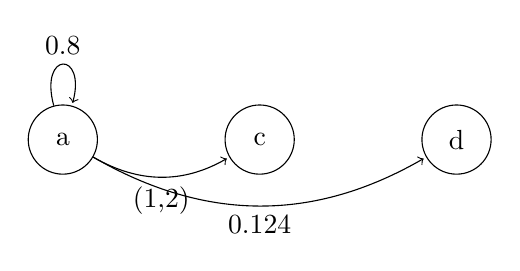
\begin{tikzpicture}

\createNode{v0}{a}{0.0}{0.0}{black}{white}
\createNode{v1}{c}{2.5}{0.0}{black}{white}
\createNode{v2}{d}{5.0}{0.0}{black}{white}
\createLoop{v0}{0.8}{black}{black}
\createEdge{v0}{v1}{(1,2)}{black}{black}
\createEdge{v0}{v2}{0.124}{black}{black}
\end{tikzpicture}
\end{document}

